\chapter{ขั้นตอนวิธีการทดสอบแบตเตอรี่ตามมาตรฐาน}
แบตเตอรี่เป็นส่วนประกอบที่มีความสำคัญมากสำหรับยานยนต์ไฟฟ้าเนื่องจากเป็นอุปกรณ์ที่กักเก็บและให้พลังงานไฟฟ้ากับยานยนต์ไฟฟ้าเพื่อความปลอดภัยของผู้ที่ใช้งานยานยนต์ไฟฟ้ามาต-รฐานต่างๆจึงถูกกำหนดขึ้นเพื่อ
ใช้กับทุกส่วนประกอบของยานยนต์ไฟฟ้ารวมถึงแบตเตอรี่ด้วยเช่นกันซึ่งการทดสอบแบตเตอรี่ที่ทางคณะผู้จัดทำได้ทำการทดสอบนั้นจะทดสอบตามมาตรฐาน UN ECE Regulation 136 ทั้งหมด 2 หัวข้อดังนี้
%\subsection{การทดสอบการป้องกันการลัดวงจรภายนอกของแบตเตอรี่}
%ในหัวข้อนี้จะเป็นการทดสอบการป้องกันการลัดวงจรภายนอกแบตเตอรี่ของแบตเตอรี่โดยจุดประสงค์ของการทดสอบนี้เพื่อทดสอบความสามารถการป้องกันการลัดวงจรของแบตเตอรี่โดยถ้าแบตเตอรี่มีอุปกรณ์ป้องกันการลัดวงจรอยู่ภาย
%ในดังนั้นอุปกรณ์ป้องกันการลัดวงจรนี้ต้องขัดจังหวะหรือจำกัดกระแสลัดวงจรเพื่อป้องกันความเสียหายที่จะเกิดขึ้นจากการลัดวงจรของแบตเตอรี่
%\newline
%\newline
%\textbf{เงื่อนไขทั่วไปในขั้นตอนการทดสอบ}
%\begin{itemize}
%{\item ระหว่างการทดสอบแบตเตอรี่ต้องทำงานอยู่ในอุณหภูมิ 20$\pm$10$^{\circ}C$ หรือสูงกว่า}
%{\item ก่อนการทดสอบแบตเตอรี่ต้องมีระดับ SOC มากกว่า 50\% ของช่วง SOC ที่แบตเตอรี่อยู่ในสภาวะการทำงานปกติ}
%{\item เมื่อเริ่มทำการทดสอบอุปกรณ์ป้องกันทุกอย่างที่ส่งผลต่อการทำงานของแบตเตอรี่ซึ่งให้ผลลัพธ์ตามจุดประสงค์ของการทดสอบจะต้องทำงาน}
%\end{itemize}
%\textbf{ขั้นตอนการทดสอบการลัดวงจร}
%\begin{itemize}
%{\item ขั้นแรกสวิตซ์ตัวนำต่างๆที่ใช้สำหรับการชาร์จและดิสชาร์จต้องปิดวงจรเพื่อจำลองถึงการใช้งานแบตเตอรี่ขณะขับขี่ยานยนต์ไฟฟ้าและการชาร์จแบตเตอรี่ภายนอกยานยนต์ไฟฟ้าถ้าหากขั้นตอนนี้ไม่สำเร็จให้ทำขั้นตอนนี้อีกครั้งจนกว่าจะสำเร็จ}
%{\item ขั้วบวกและขั้วลบของแบตเตอรี่จะต้องทำการเชื่อมต่อถึงกันและกันเพื่อให้เกิดการลัดวงจรโดยอุปกรณ์การเชื่อมต่อนี้จะต้องมีความต้านทานไม่เกิน 5 มิลลิโอห์ม}
%{\item การลัดวงจรจะถูกดำเนินไปอย่างต่อเนื่องจนกว่าจะถูกขัดจังหวะจากการทำงานของแบตเตอรี่หรือมีการจำกัดกระแสลัดวงจร หรือต้องมีการวัดอุณหภูมิที่ตัวแบตเตอรี่เป็นเวลาอย่างน้อย 1 ชั่วโมงโดยตลอดระยะเวลาที่ทำการวัดอุณหภูมิต้องมีการเปลี่นแปลงไม่เกิน 4$^{\circ}C$}
%{\item การทดสอบจะยุติลงหลังจากการสังเกตการแบตเตอรี่ที่อุณหภูมิตามเงื่อนไขข้างต้นตามสภาพแวดล้อมที่ใช้ในการทดสอบ}
%\end{itemize}
%=======================================================================================================
\subsection{การทดสอบการป้องกันการชาร์จเกินของแบตเตอรี่}
สำหรับหัวข้อการทดสอบนี้จะเป็นการทดสอบการป้องกันการชาร์จไฟฟ้าเกินขีดจำกัดของแบตเตอรี่เพื่อเป็นการทดสอบประสิทธิภาพการป้องกันการชาร์จเกินขีดจำกัดของแบตเตอรี่
\newline
\newline
\textbf{เงื่อนไขทั่วไปในขั้นตอนการทดสอบ}
\begin{itemize}
{\item ระหว่างการทดสอบแบตเตอรี่ต้องทำงานอยู่ในอุณหภูมิ 20$\pm$10$^{\circ}C$ หรือสูงกว่า}
{\item เมื่อเริ่มทำการทดสอบอุปกรณ์ป้องกันทุกอย่างที่ส่งผลต่อการทำงานของแบตเตอรี่ซึ่งให้ผลลัพธ์ตามจุดประสงค์ของการทดสอบจะต้องทำงาน}
\end{itemize}
\textbf{ขั้นตอนการทดสอบการชาร์จ}
\begin{itemize}
{\item ขั้นแรกสวิตซ์ตัวนำต่างๆที่ใช้สำหรับการชาร์จต้องปิดวงจร}
{\item อุปกรณ์ควบคุมจำกัดการชาร์จของอุปกรณ์วัดหรืออุปกรณ์ทดสอบแบตเตอรี่ต้องถูกปิดการใช้งาน}
{\item แบตเตอรี่ต้องถูกชาร์จด้วยอัตรากระแสอย่างน้อย 1/3 C แต่ต้องไม่เกินกระแสสูงสุดในช่วงการทำงานปกติตามที่ผู้ผลิตแบตเตอรี่ได้กำหนดไว้}
{\item การชาร์จจะถูกดำเนินไปอย่างต่อเนื่องจนกว่าการชาร์จจะถูกขัดจังหวะจากการทำงานของแบตเตอรี่หรือการชาร์จถึงขีดจำกัด เมื่อการขัดจังหวะโดยการทำงานของแบตเตอรี่นั้นไม่ทำงานหรือตัวแบตเตอรี่ไม่มีการทำงานในส่วนของการขัดจังหวะนี้การชาร์จจะถูกดำเนินต่อไปเรื่อยๆจนกว่าจะชาร์จถึง 2 เท่าของความจุพิกัด}
{\item การทดสอบจะยุติลงหลังจากการสังเกตการแบตเตอรี่ที่อุณหภูมิตามเงื่อนไขข้างต้นตามสภาพแวดล้อมที่ใช้ในการทดสอบ}
\end{itemize}
%=======================================================================================================
\subsection{การทดสอบการป้องกันการดิสชาร์จเกินของแบตเตอรี่}
ในการทดสอบการป้องกันการดิสชาร์จเกินโดยวัตถุประสงค์ของการทดสอบนี้เพื่อทดสอบความสามารถในการป้องกันการดิสชาร์จเกินของแบตเตอรี่โดยถ้าแบตเตอรี่มีอุปกรณ์ป้องกันการชาร์จเกินอยู่ภายในดังนั้นอุปกรณ์ป้องกันการชาร์จเกิน
นี้ต้องขัดจังหวะหรือจำกัดกระแสการดิสชาร์จเพื่อป้องกันความเสียหายต่างๆเนื่องจากค่า SOC ที่ต่ำเกินกว่าที่ผู้ผลิตแบตเตอรี่ได้กำหนดเอาไว้
\newline
\newline
\textbf{เงื่อนไขทั่วไปในขั้นตอนการทดสอบ}
\begin{itemize}
{\item ระหว่างการทดสอบแบตเตอรี่ต้องทำงานอยู่ในอุณหภูมิ 20$\pm$10$^{\circ}C$ หรือสูงกว่า}
{\item เมื่อเริ่มทำการทดสอบอุปกรณ์ป้องกันทุกอย่างที่ส่งผลต่อการทำงานของแบตเตอรี่ซึ่งให้ผลลัพธ์ตามจุดประสงค์ของการทดสอบจะต้องทำงาน}
\end{itemize}
\textbf{ขั้นตอนการทดสอบการดิสชาร์จ}
\begin{itemize}
{\item ขั้นแรกสวิตซ์ตัวนำต่างๆที่ใช้สำหรับการดิสชาร์จต้องปิดวงจร}
{\item อุปกรณ์ควบคุมจำกัดการชาร์จของอุปกรณ์วัดหรืออุปกรณ์ทดสอบแบตเตอรี่ต้องถูกปิดการใช้งาน}
{\item แบตเตอรี่ต้องถูกดิสชาร์จด้วยอัตรากระแสอย่างน้อย 1/3 C แต่ต้องไม่เกินกระแสสูงสุดในช่วงการทำงานปกติตามที่ผู้ผลิตแบตเตอรี่ได้กำหนดไว้}
{\item การดิสชาร์จจะถูกดำเนินไปอย่างต่อเนื่องจนกว่าการดิสชาร์จจะถูกขัดจังหวะจากการทำงานของแบตเตอรี่หรือการดิสชาร์จถึงขีดจำกัด เมื่อการขัดจังหวะโดยการทำงานของแบตเตอรี่นั้นไม่ทำงานหรือตัวแบตเตอรี่ไม่มีการทำงานในส่วนของการขัดจังหวะนี้การดิสชาร์จจะถูกดำเนินต่อไปเรื่อยๆจนกว่าแบตเตอรี่จะถูกดิสชาร์จจนถึง 25\% ของระดับแรงดันปกติ}
{\item หลังหยุดการดิสชาร์จแล้วแบตเตอรี่จะต้องนำไปชาร์จใหม่ด้วยอัตรากระแสปกติตามที่ผู้ผลิตได้กำหนดไว้ถ้าหากไม่ได้มีการกำหนดจะต้องทำการชาร์จด้วยอัตรากระแส 1/3 C}
{\item การทดสอบจะยุติลงหลังจากการสังเกตการแบตเตอรี่ที่อุณหภูมิตามเงื่อนไขข้างต้นตามสภาพแวดล้อมที่ใช้ในการทดสอบ}
\end{itemize}
%========================================================================================================
โดยทั้ง 2 หัวข้อของการทดสอบตามมาตรฐาน UN ECE Regulation 136 นั้นเงื่อนไขที่จะผ่านการทดสอบแบตเตอรี่มีดังนี้
\begin{enumerate}
{\item ในระหว่างการทดสอบแบตเตอรี่จะต้องไม่มีอิเล็กโทรไลต์รั่วไหลออกจากแบตเตอรี่ โดยการสังเกตการรั่วไหลของอิเล็กโทรไลต์ให้สังเกตโดยรอบของแบตเตอรี่เพียงเท่านั้นโดยไม่ต้องแยกชิ้นส่วนใดๆของแบตเตอรี่ออก}
{\item ในระหว่างการทดสอบแบตเตอรี่จะต้องไม่เกิดการแตกหักหรือฉีกขาด}
{\item ในระหว่างการทดสอบแบตเตอรี่จะต้องไม่เกิดเพลิงไหม้}
{\item ในระหว่างการทดสอบแบตเตอรี่จะต้องไม่เกิดการระเบิด}
\end{enumerate}
%========================================================================================================
\section{ขั้นตอนการทดสอบอื่นๆ}
สำหรับการทดสอบอื่นที่นอกเหนือจากทดสอบตามาตรฐานนี้จะทดสอบด้วยกันทั้งหมด 3 หัวข้อคือ
\begin{itemize}
{\item การทดสอบระยะเวลาในการพัก}
{\item การทดสอบอัตรากระแส}
{\item การทดสอบการวัดค่าความต้านทานภายในของโมดูลแบตเตอรี่}
\end{itemize}
\subsection{การทดสอบระยะเวลาในการพักของแบตเตอรี่}
สำหรับการทดสอบนี้จะทดสอบเพื่อหาระยะเวลาในการพักแบตเตอรี่ที่เหมาะสมที่สุดที่แบตเตอรี่จะไม่เกิดการเปลี่ยนแปลงโดยขั้นตอนการทดสอบมีดังนี้
\begin{enumerate}
{\item ทำการชาร์จแบตเตอรี่ด้วยวิธีกระแสงที่แรงดันคงที่(CC-CV) จนกระทั้งแรงดันถึง 80\%SOC}
{\item เมื่อชาร์จแบตเตอรี่แล้วทำการพักเพื่อสังเกต 3 ชั่วโมง}
{\item ทำการดิสชาร์จด้วยวิธีกระแสคงที่(CC) จนกระทั่งแรงดันถึง 20\%SOC}
{\item เมื่อดิสชาร์จแบตเตอรี่แล้วทำการพักเพื่อสังเกต 3 ชั่วโมง}
\end{enumerate}
\subsection{การทดสอบอัตรากระแส}
สำหรับการทดสอบนี้จะทดสอบเพื่อศึกษาอัตรากระแสนั้นมีผลต่อแรงดันและความจุอย่างไร
\begin{enumerate}
{\item ทำการชาร์จแบตเตอรี่ด้วยวิธีกระแสงที่แรงดันคงที่(CC-CV) จนกระทั้งแรงดันถึง 80\%SOC}
{\item เมื่อชาร์จแบตเตอรี่แล้วทำการพัก 30 นาที}
{\item ทำการดิสชาร์จด้วยวิธีกระแสคงที่(CC) จนกระทั่งแรงดันถึง 20\%SOC}
{\item เมื่อดิสชาร์จแบตเตอรี่แล้วทำการพักเพื่อสังเกต 30 นาที}
{\item ทำซ้ำตั้งแต่ขั้นตอนแรก}
\end{enumerate}
โดยจะทดสอบทั้งหมดตามขั้นตอนนี้ 3 ครั้งโดยแต่ละครั้งจะเปลี่ยนอัตรากระแสการดิสชาร์จคือ 0.2C 0.3C และ 0.5C
\subsection{การทดสอบวัดค่าความต้านทานภายในของแบตเตอรี่}
การทดสอบนี้จะเป็นการทดสอบการวัดค่าความต้านทานภายในของแบตเตอรี่ด้วยไฟฟ้ากระแสตรง(Direct Current Internal Resistance,DCIR)
จากมาตรฐาน IEC61960 ขั้นตอนการทดสอบคือ
\begin{enumerate}
{\item ดิสชาร์จด้วยกระแสคงที่ 0.2C เป็นระยะเวลา 10 วินาที}
{\item ดิสชาร์จด้วยกระแสคงที่ 1C เป็นระยะเวลา 1 วินาที}
\end{enumerate}
จากนั้นสังเกตและบันทึกค่าแรงดันที่เปลี่ยนแปลงต่ออัตรากระแสที่เปลี่ยนแปลงจากนั้นนำมาวิเคราะห์ดังสมการ
$ DCIR = \frac{V_2-V_1}{I_1-I_2} $
%========================================================================================================
\section{อุปกรณ์สำหรับทดสอบแบตเตอรี่}
ในการทดสอบแบตเตอรี่สำหรับโครงงานนี้อุปกรณ์หลักที่จะใช้ในการทดสอบในหัวข้อต่างๆคือเครื่องทดสอบแบตเตอรี่ Chroma Model 17020 โดยอุปกรณ์ที่ใช้ในระบบของเครื่องนี้ประกอบด้วย
\begin{enumerate}
{\item 69200-1 Charge/Discharge Controller \newline
ทำหน้าที่เก็บข้อมูลการทดสอบแบตเตอรี่ทุกๆ 1 วินาทีและสามารถควบคุมการทำงานผ่านระบบอีเทอร์เน็ต(Ethernet)ได้}
{\item A691101 DC/AC Bi-Direction Converter\newline
ทำหน้าที่แปลงกระแสไฟฟ้าเป็นไฟฟ้ากระแสตรงให้กับเครื่องทดสอบและสามารถแปลงกระแสไฟฟ้ากระแสตรงจากแบตเตอรี่ให้เป็นกระแสสลับเพื่อนำกลับมาใช้ใหม่}
{\item 69225-100-4 Regenerative Charge/Discharge Tester\newline
ทำหน้าที่จ่ายพลังงานไฟฟ้าให้กับแบตเตอรี่หรือรับพลังงานไฟฟ้าจากแบตเตอรี่}
{\item ON/OFF Controller\newline
ทำหน้าที่ควบคุมการจ่ายพลังงานไฟฟ้าให้กับระบบของเครื่องทดสอบแบตเตอรี่}
\end{enumerate}
\begin{center}
	\begin{figure}[H]
		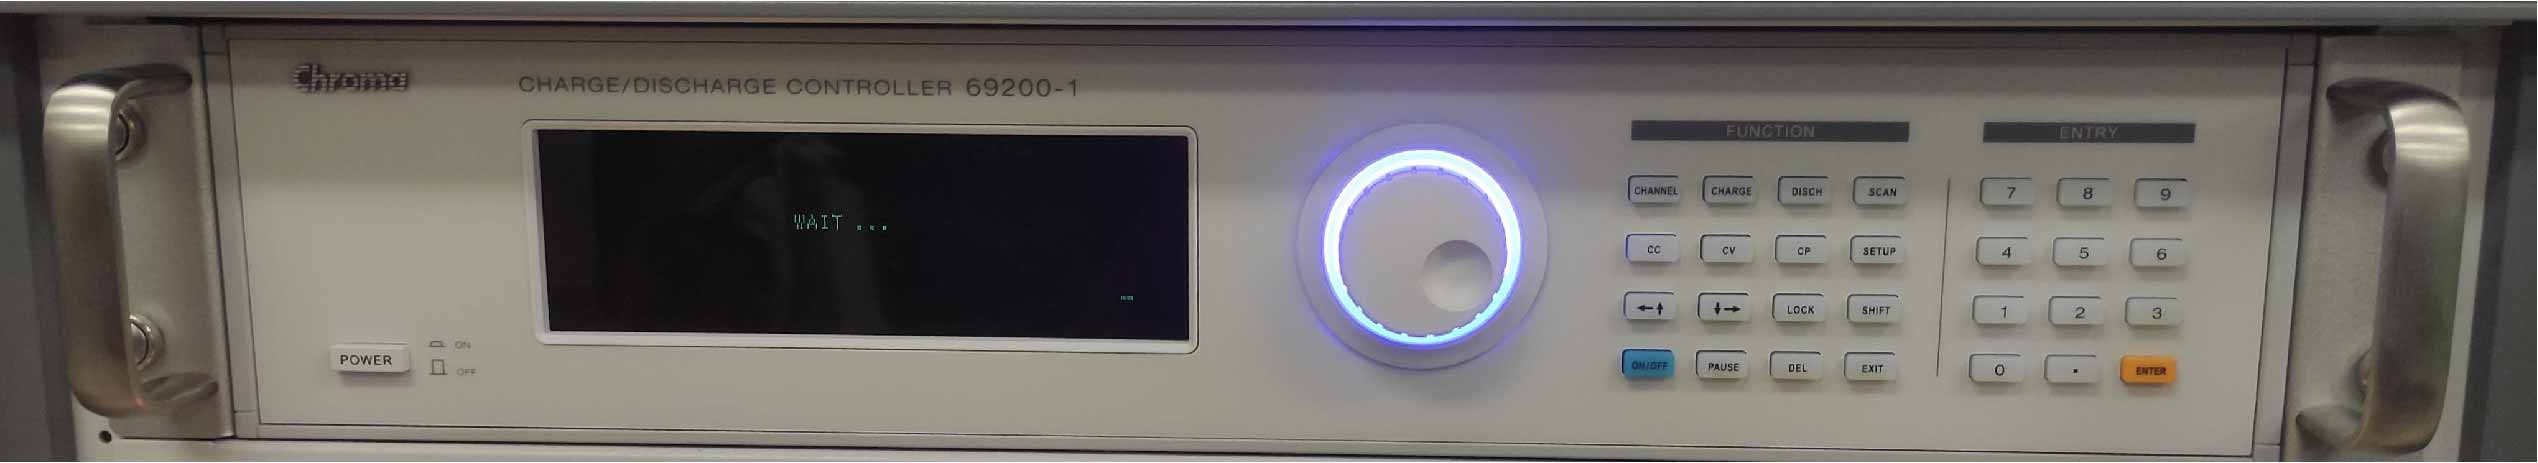
\includegraphics[width=1\linewidth]{Chapters/img/Charge_Discharge_Controller.jpg}
			\centering
			\captionsetup{justification=centering,margin=2cm}
			\caption{Charge/Discharge Controller}
	\end{figure}
	\begin{figure}[H]
		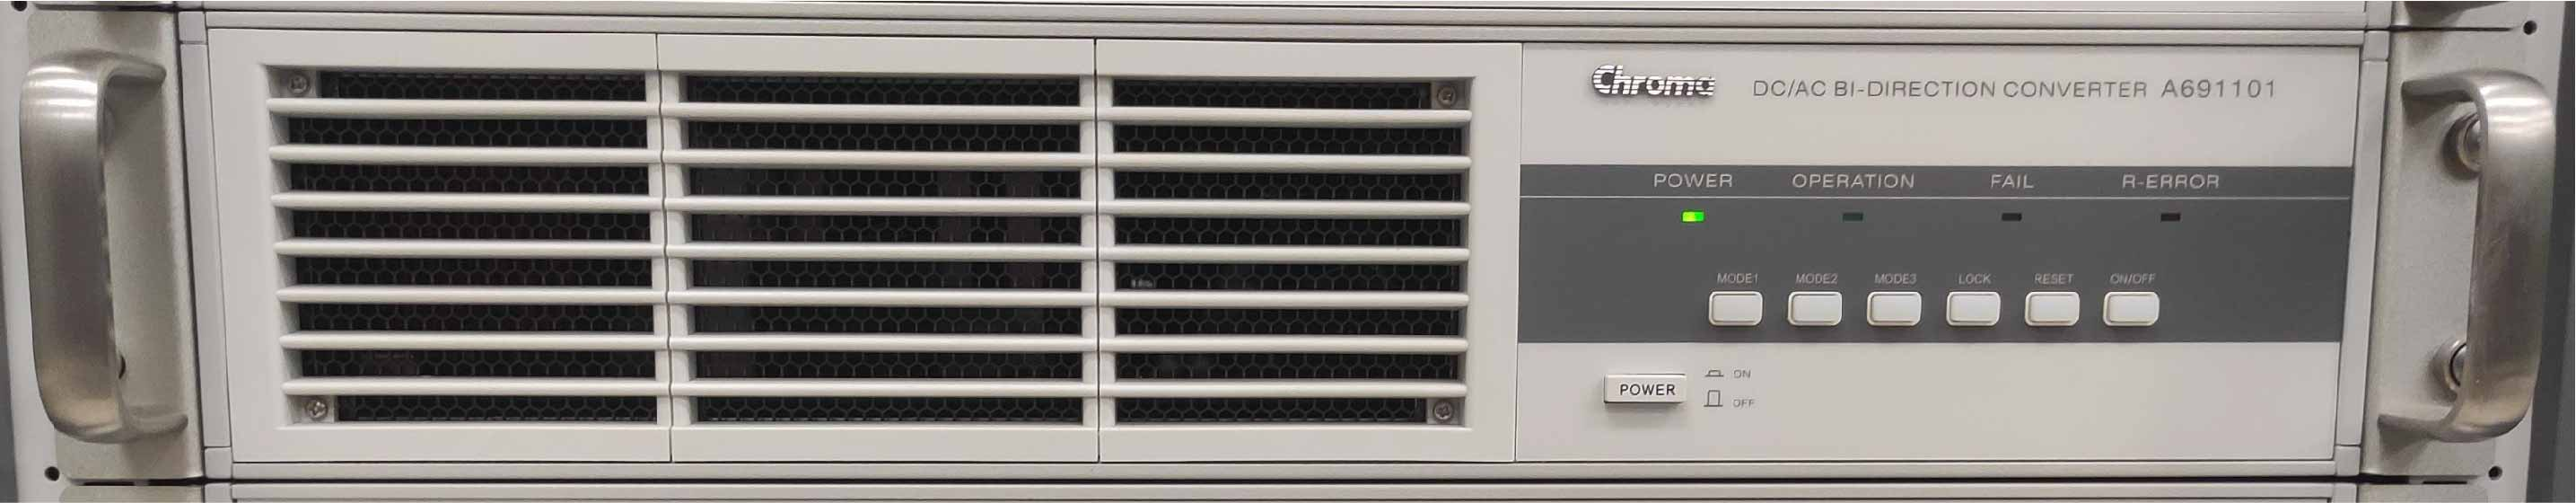
\includegraphics[width=1\linewidth]{Chapters/img/Bi_Direction_Converter.jpg}
			\centering
			\captionsetup{justification=centering,margin=2cm}
			\caption{DC/AC Bi-Direction Converter}
	\end{figure}
	\begin{figure}[H]
		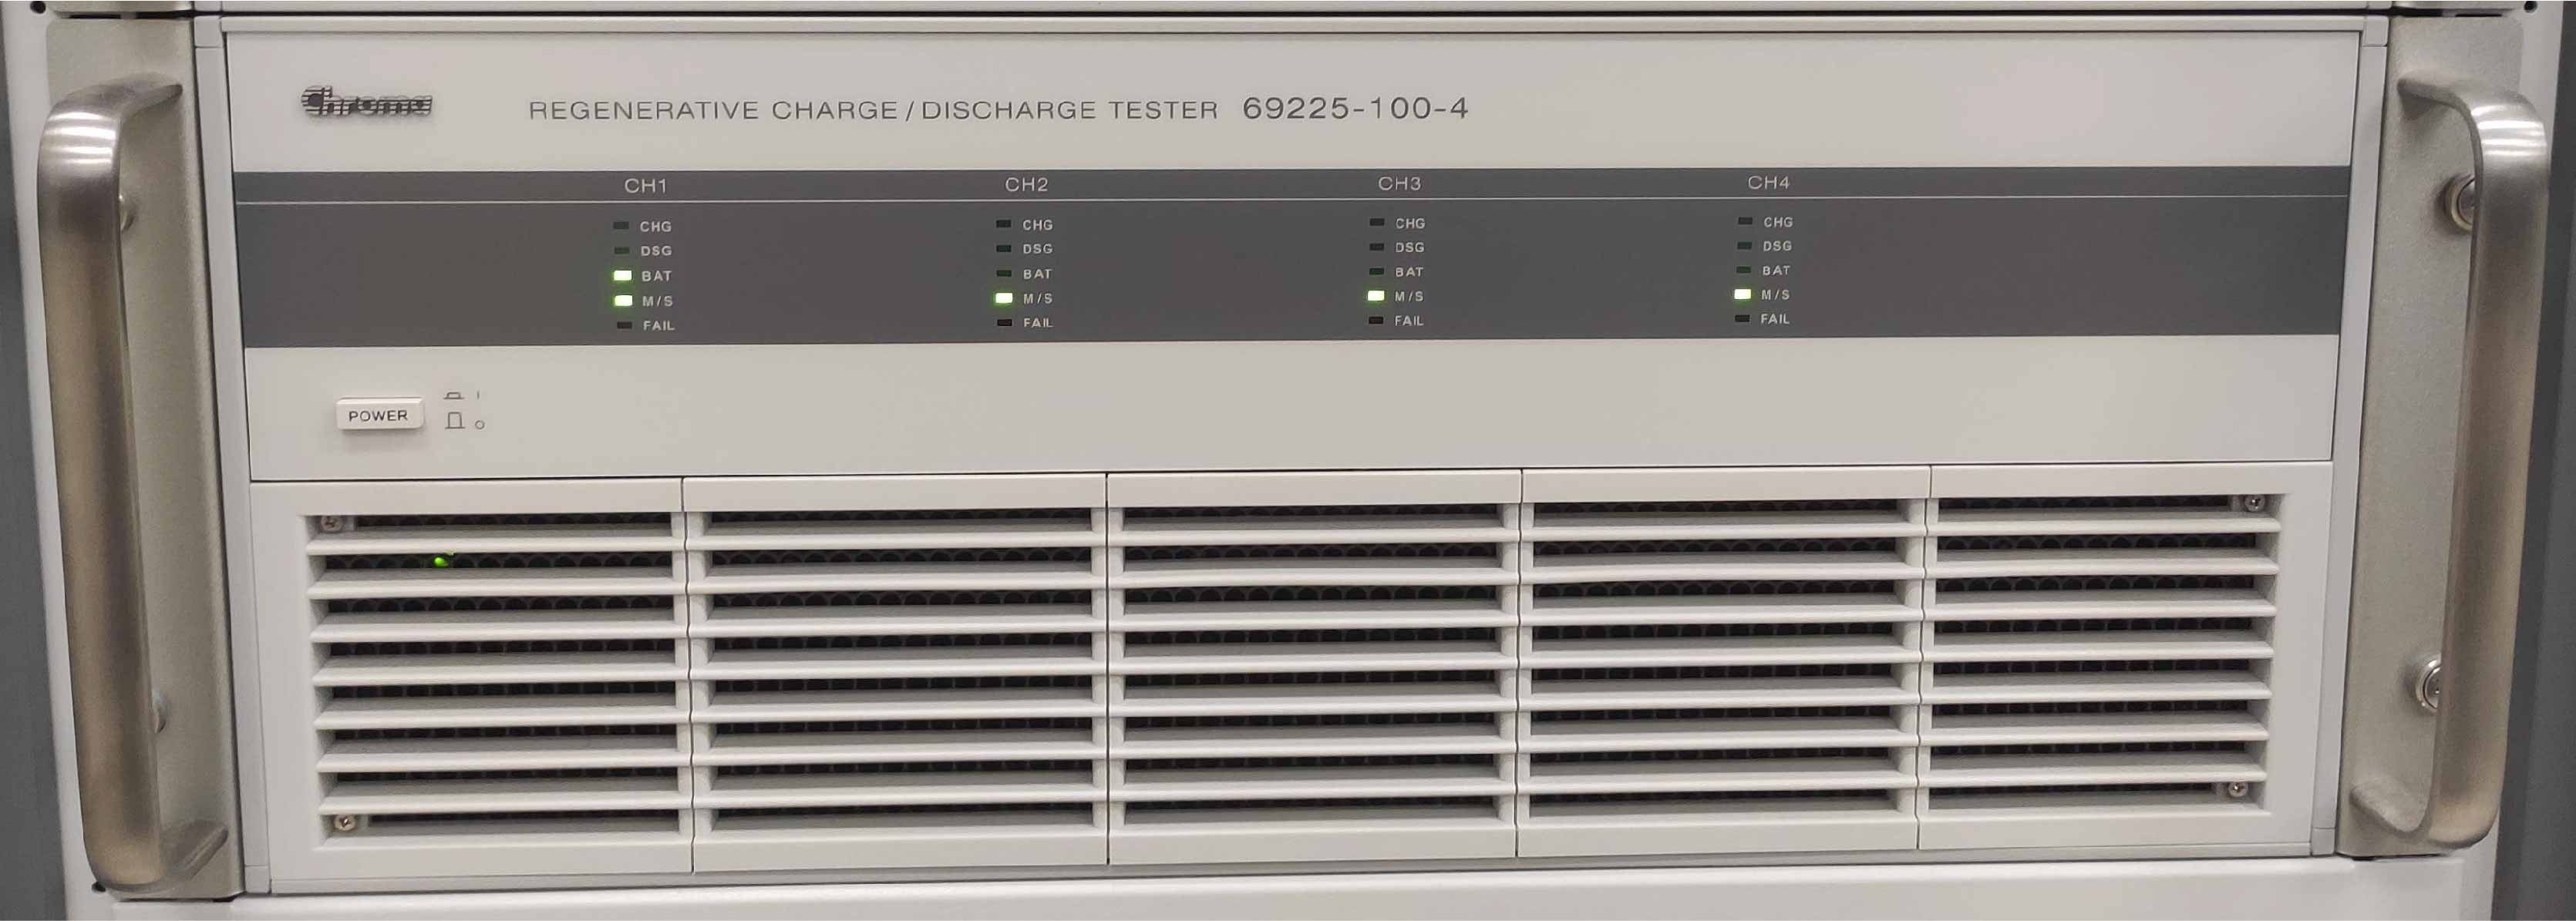
\includegraphics[width=1\linewidth]{Chapters/img/Regenerative_Charge_Discharge.jpg}
			\centering
			\captionsetup{justification=centering,margin=2cm}
			\caption{Regenerative Charge/Discharge Tester}
	\end{figure}
	\begin{figure}[H]
		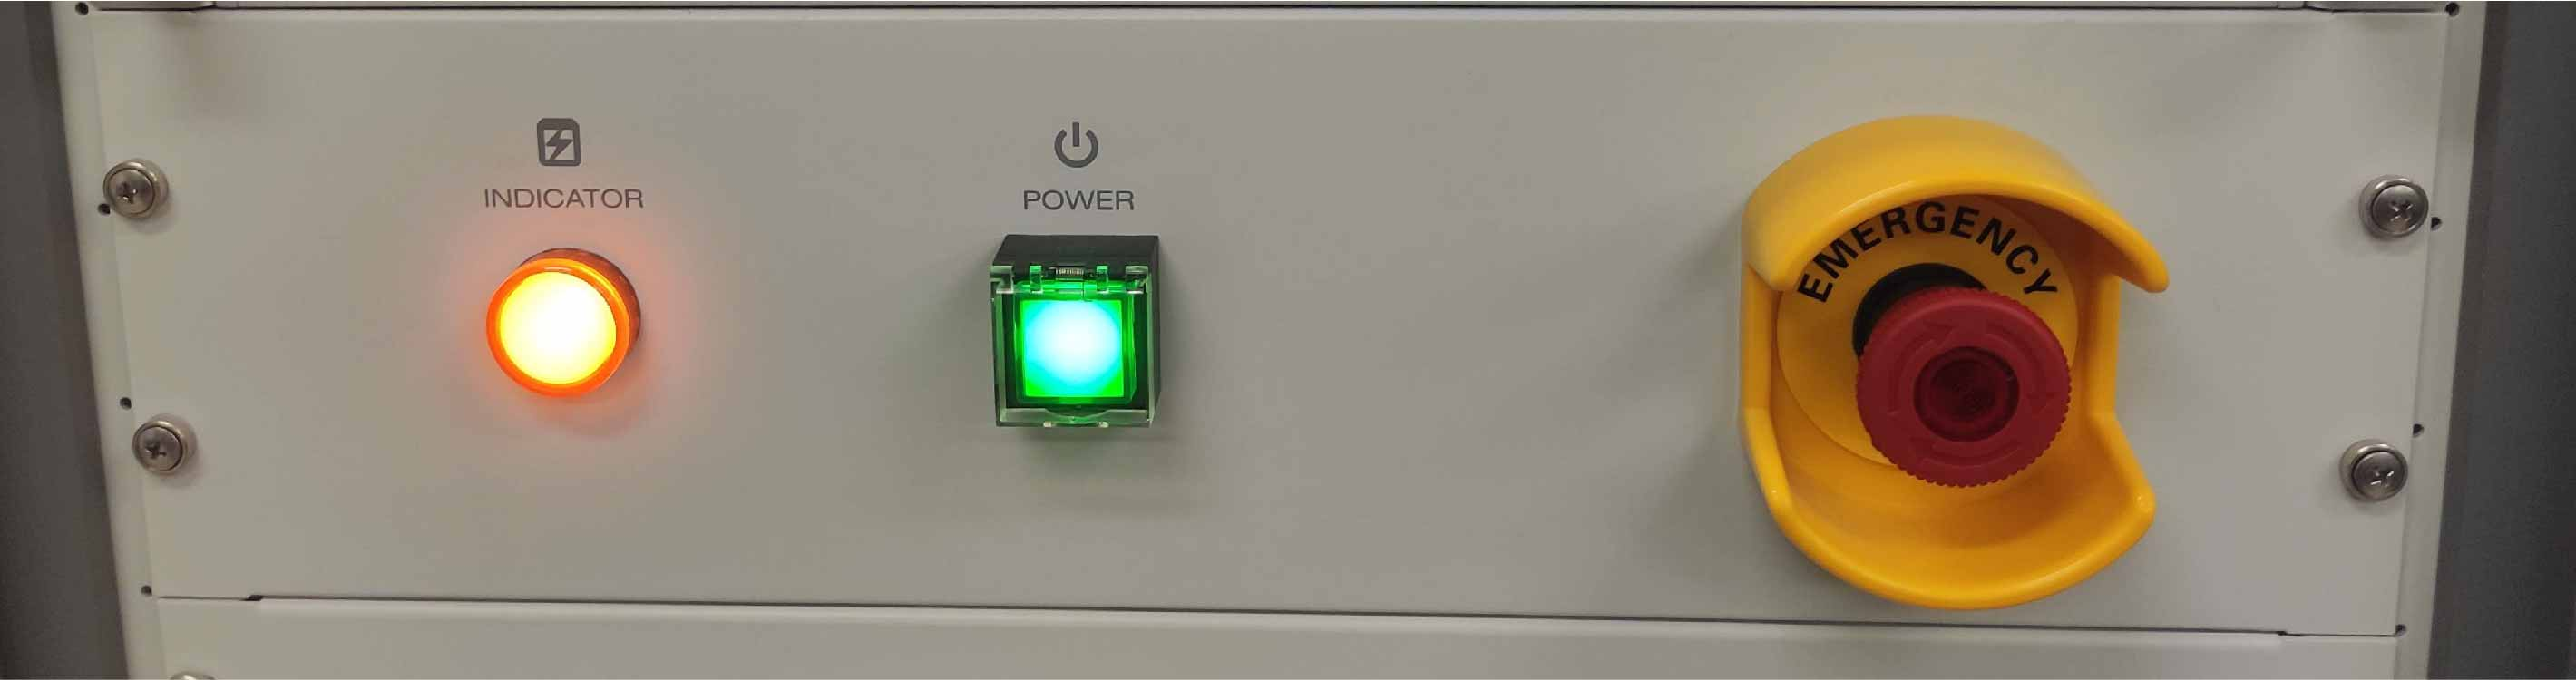
\includegraphics[width=1\linewidth]{Chapters/img/ON_OFF_Controller.jpg}
			\centering
			\captionsetup{justification=centering,margin=2cm}
			\caption{ON/OFF Controller}
	\end{figure}
%	\begin{figure}[!h]
%		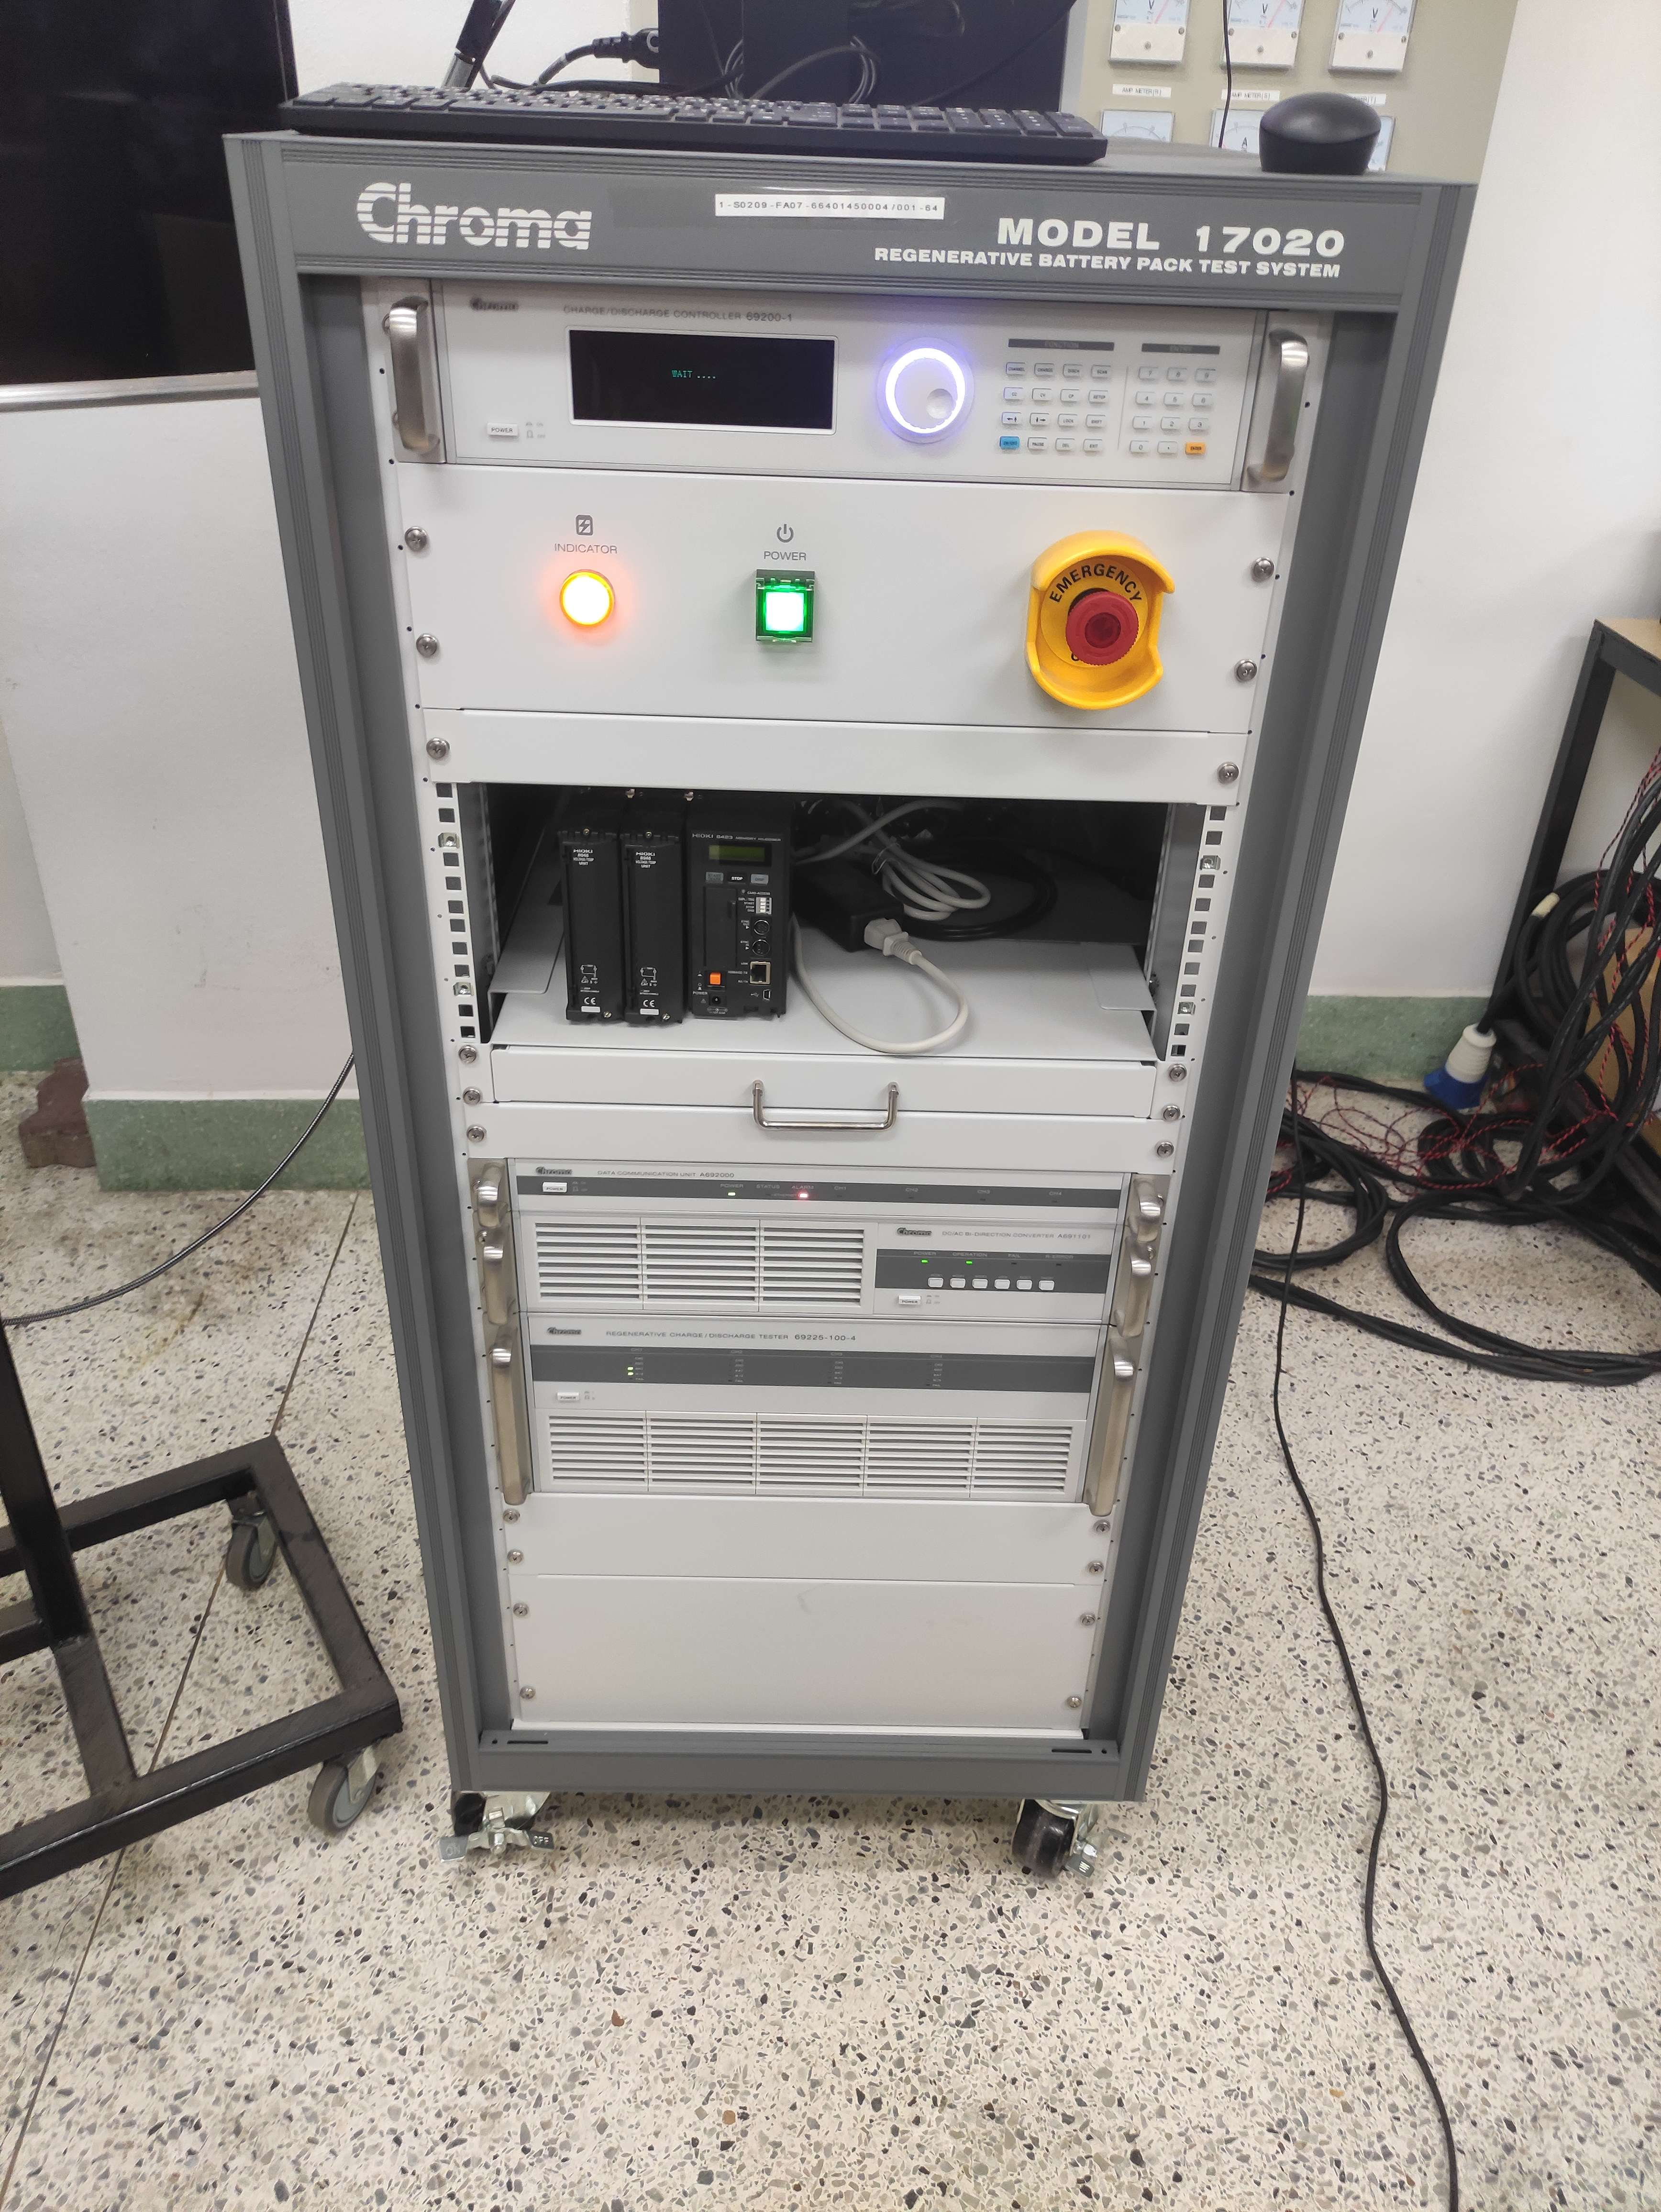
\includegraphics[width=0.5\linewidth]{Chapters/img/Chroma_17020_3.jpg}
%			\centering
%			\captionsetup{justification=centering,margin=2cm}
%			\caption{เครื่องทดสอบแบตเตอรี่ Chroma Model 17020}
%	\end{figure}
\begin{figure}[!h]
	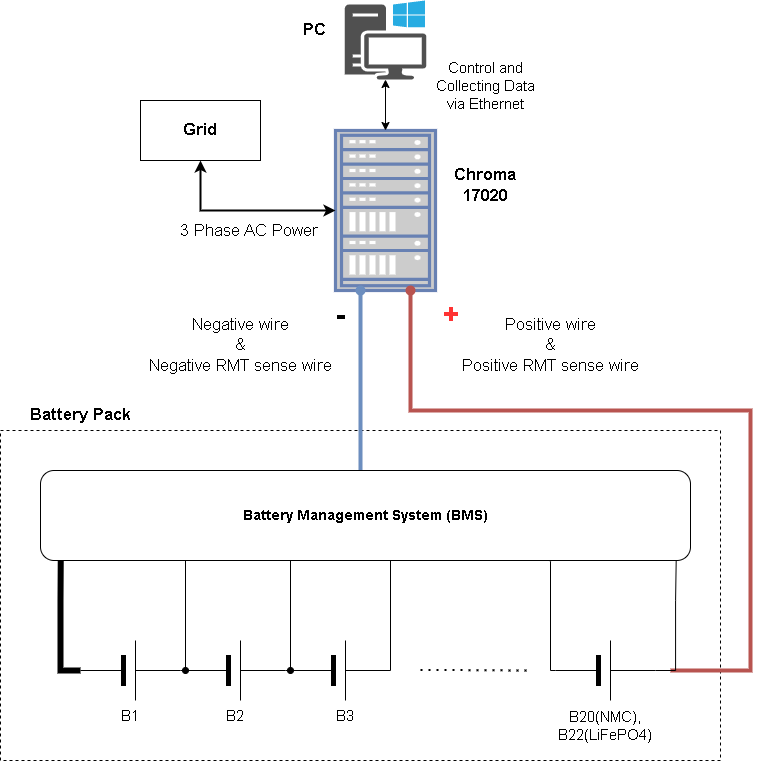
\includegraphics[width=1\linewidth]{Chapters/img/Testing_System.png}
		\centering
		\captionsetup{justification=centering,margin=2cm}
		\caption{แผนภาพระบบการทดสอบแบตเตอรี่}
	\end{figure}
\end{center}
%========================================================================
\vfill
\subsection{แบตเตอรี่สำหรับทำการทดสอบ}
แบตเตอรี่ที่ทำการทดสอบเป็นแบตเตอรี่ชนิดลิเธียมแมงกานีสโคบอลท์ออกไซด์(NMC)พิกัด 72V/30Ah ซึ่งคุณสมบัติแสดงดังตาราง
\begin{center}
	\begin{figure}[H]
		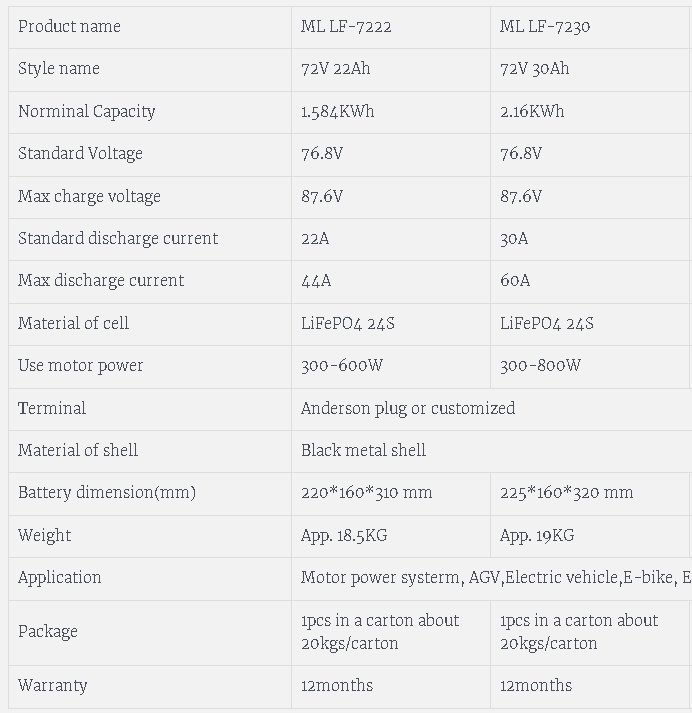
\includegraphics[width=0.5\linewidth]{Chapters/img/Battery_name_plate.PNG}
		\centering
		\captionsetup{justification=centering,margin=2cm}
		\caption{ตารางคุณสมบัติของแบตเตอรี่}
	\end{figure}
	\begin{figure}[H]
		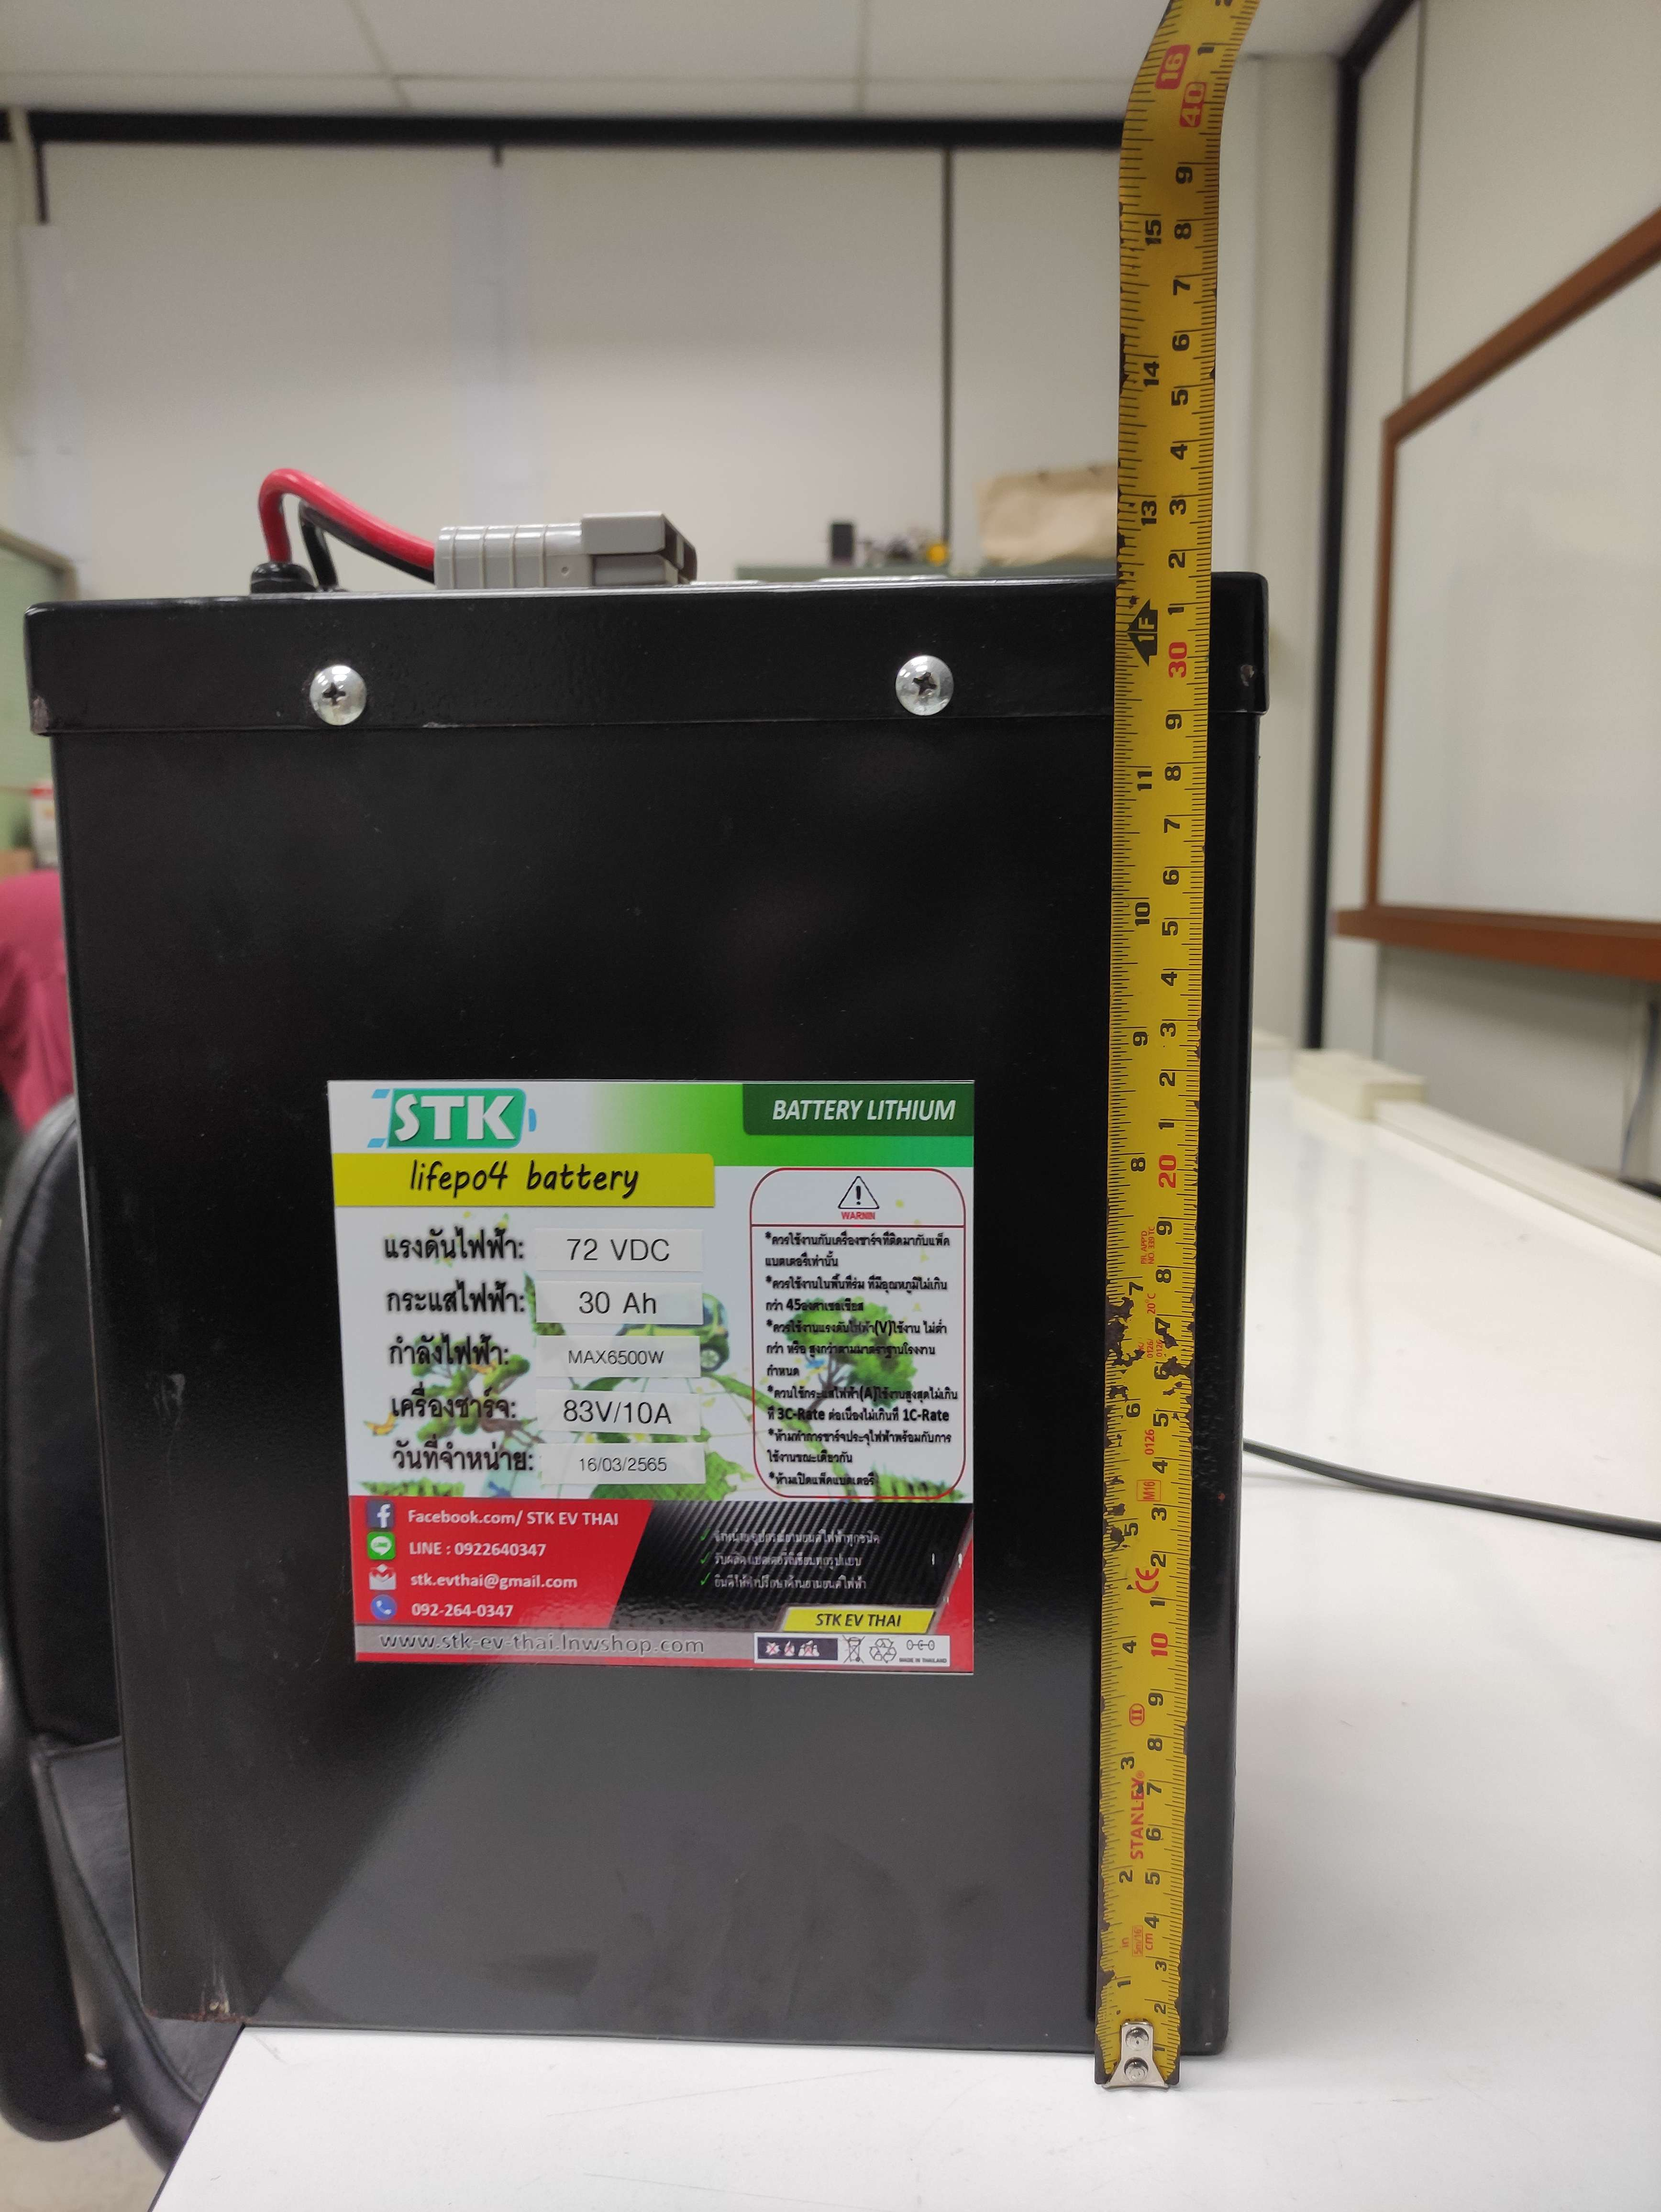
\includegraphics[width=0.5\linewidth]{Chapters/img/Battery_72V_30AH}
		\centering
		\captionsetup{justification=centering,margin=2cm}
		\caption{แบตเตอรี่สำหรับทำการทดสอบ}
	\end{figure}
\end{center}
%========================================================================================================
โดยใช้งานเครื่องทดสอบแบตเตอรี่ในการทดสอบแบตเตอรี่ในแต่ละหัวข้อมีดังนี้
%========================================================================================================
%\subsection{การใช้เครื่องทดสอบแบตเตอรี่ Chroma Model 17020 \\ ในการทดสอบการป้องกันการลัดวงจรภายนอกของแบตเตอรี่}
%สำหรับหัวข้อการทดสอบการป้องกันการลัดวงจรภายนอกของแบตเตอรี่
%========================================================================================================
\subsection{การใช้เครื่องทดสอบแบตเตอรี่ Chroma Model 17020 \\ ในการทดสอบการป้องกันการชาร์จเกินของแบตเตอรี่}
สำหรับหัวข้อการทดสอบการป้องกันการชาร์จเกินของแบตเตอรี่โดยใช้เครื่องทดสอบแบตเตอรี่ Chroma Model 17020 ในการทดสอบพารามิเตอร์ต่างๆจะถูกตั้งค่าให้เหมาะสมสำหรับการทดสอบตามมาตรฐาน UN ECE Regulation 136 โดยให้เครื่องทดสอบแบตเตอรี่ทำการชาร์จแบตเตอรี่ด้วยโหมดแรงดันและกระแสคงที่(CC-CV)ที่แรงดัน 84V และอัตรากระแส 1/3C หรือสำหรับแบตเตอรี่ที่ใช้สำหรับการทดสอบนี้คือ 10A
และจะชาร์จจนกว่าระบบป้องกันการชาร์จเกินของแบตเตอรี่ในที่นี้คือระการจัดการแบตเตอรี่(BMS)จะทำการขัดจังหวะการชาร์จเพื่อป้องกันการดิสชาร์จเกินของแบตเตอรี่โดยขณะที่ระบบป้องกันของเครื่องทดสอบแบตเตอรี่จะป้องกันในเรื่องของ
ป้องกันกระแสชาร์จเกิน12A ป้องกันแรงดันสูงเกิน2เท่าของแรงดันพิกัดแบตเตอรี่ที่ใช้ทำการทดสอบในที่นี้คือ 170V และป้องกันแรงดันต่ำเกิน 50\% SOC หรือในที่นี้คือ 36V โดยการตั้งค่าต่างๆจะเป็นไปดังรูป
\begin{center}
	\begin{figure}[H]
		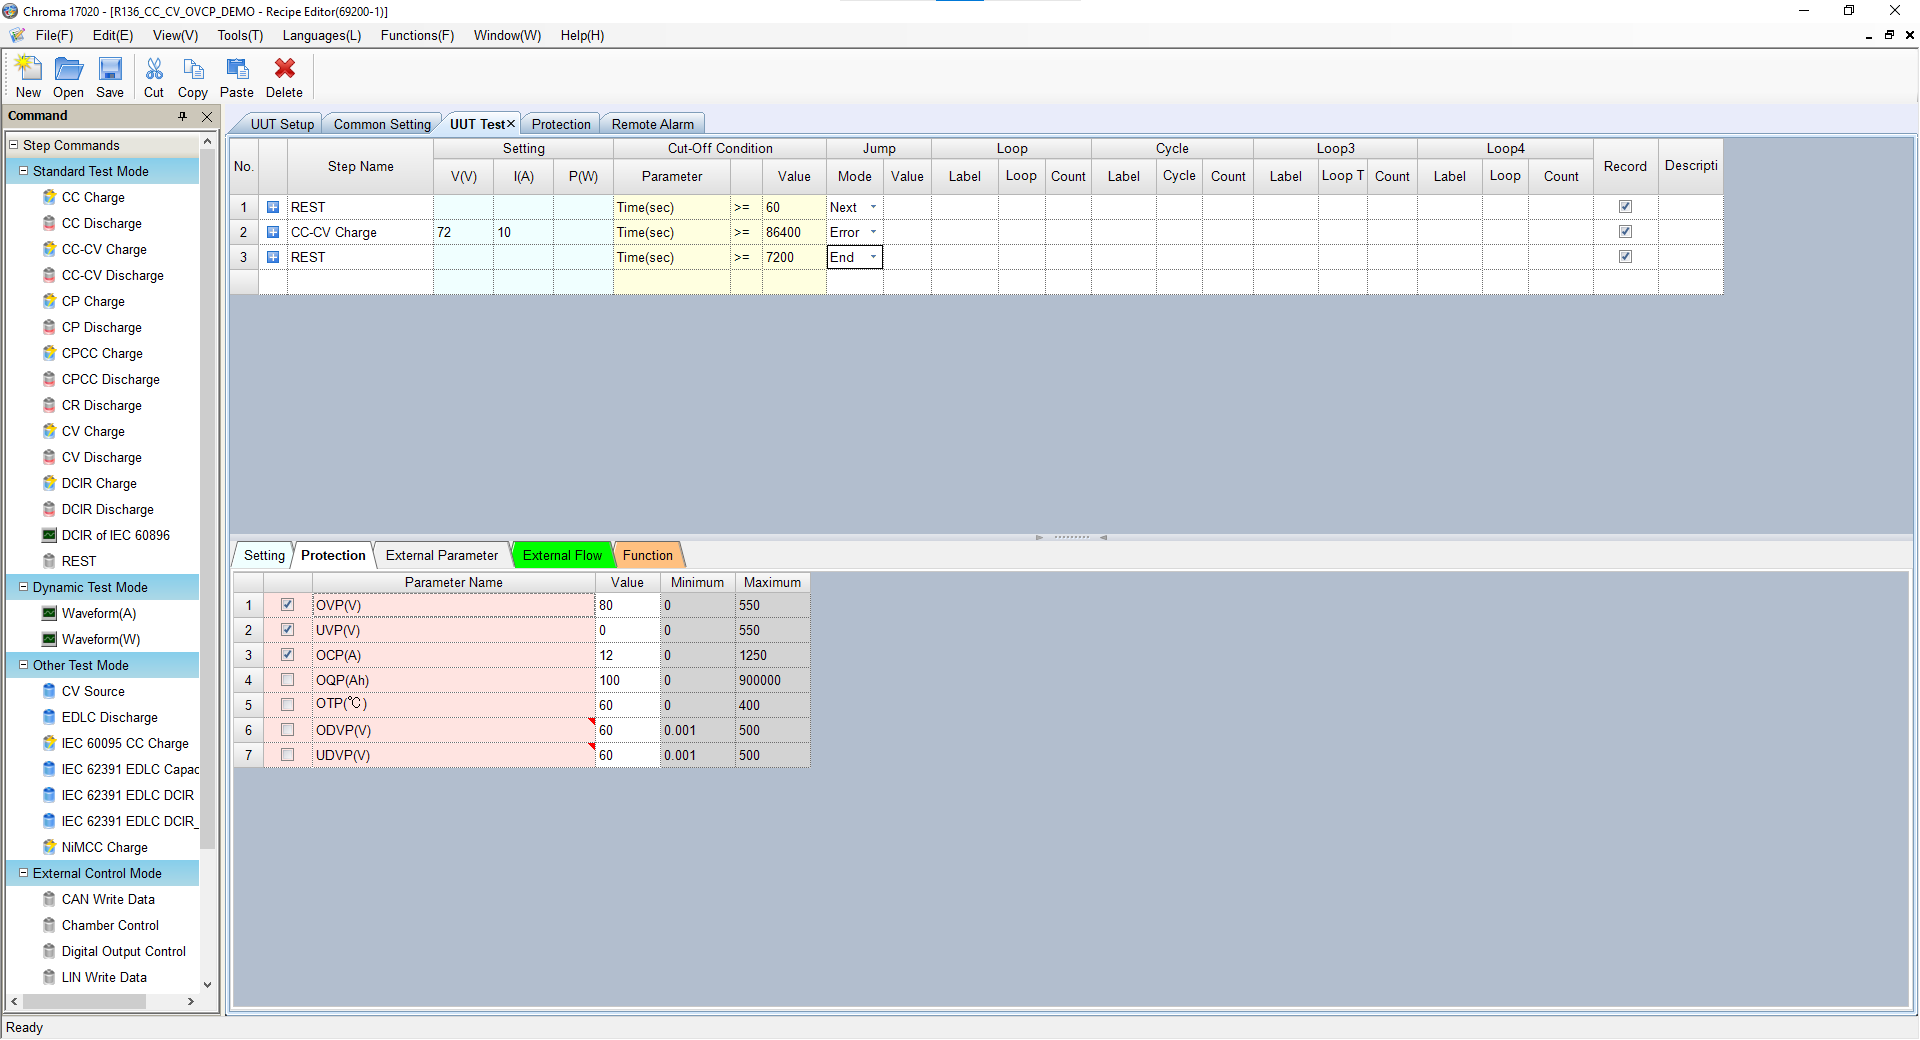
\includegraphics[width=1\linewidth]{Chapters/img/R136_DEMO/UUT_TEST_OVCP.png}
		\centering
		\captionsetup{justification=centering,margin=2cm}
		\caption{การตั้งค่าสำหรับการทดสอบการป้องกันการชาร์จเกินของแบตเตอรี่}
	\end{figure}
\end{center}
%========================================================================================================
\subsection{การใช้เครื่องทดสอบแบตเตอรี่ Chroma Model 17020 \\ ในการทดสอบการป้องกันการดิสชาร์จเกินของแบตเตอรี่}
ในการทดสอบการป้องกันการดิสชาร์จเกินของแบตเตอรี่โดยใช้เครื่องทดสอบแบตเตอรี่ Chroma Model 17020 ในการทดสอบพารามิเตอร์ต่างๆจะถูกตั้งค่าให้เหมาะสมสำหรับการทดสอบตามมาตรฐาน UN ECE Regulation 136 โดยให้เครื่องทดสอบแบตเตอรี่ทำการดิสชาร์จแบตเตอรี่ด้วยโหมดกระแสคงที่(CC)ด้วยอัตรา 1/3C หรือสำหรับแบตเตอรี่ที่จะทำการทดสอบก็คือกระแสขนาด 10A โดยจะดิสชาร์จต่อเนื่องจนกว่า
ระบบป้องกันการดิสชาร์จเกินของแบตเตอรี่ในที่นี้คือระการจัดการแบตเตอรี่(BMS)จะทำการขัดจังหวะการดิสชาร์จเพื่อป้องกันการดิสชาร์จเกินของแบตเตอรี่โดยขณะที่ระบบป้องกันของเครื่องทดสอบแบตเตอรี่จะป้องกันในเรื่องของ
ป้องกันกระแสดิสชาร์จเกิน12A ป้องกันแรงดันต่ำเกิน 24\% SOC หรือในที่นี้คือ 17.28V และป้องกันแรงดันเกิน 85V โดยการตั้งค่าต่างๆจะเป็นไปดังรูป
\begin{center}
	\begin{figure}[H]
		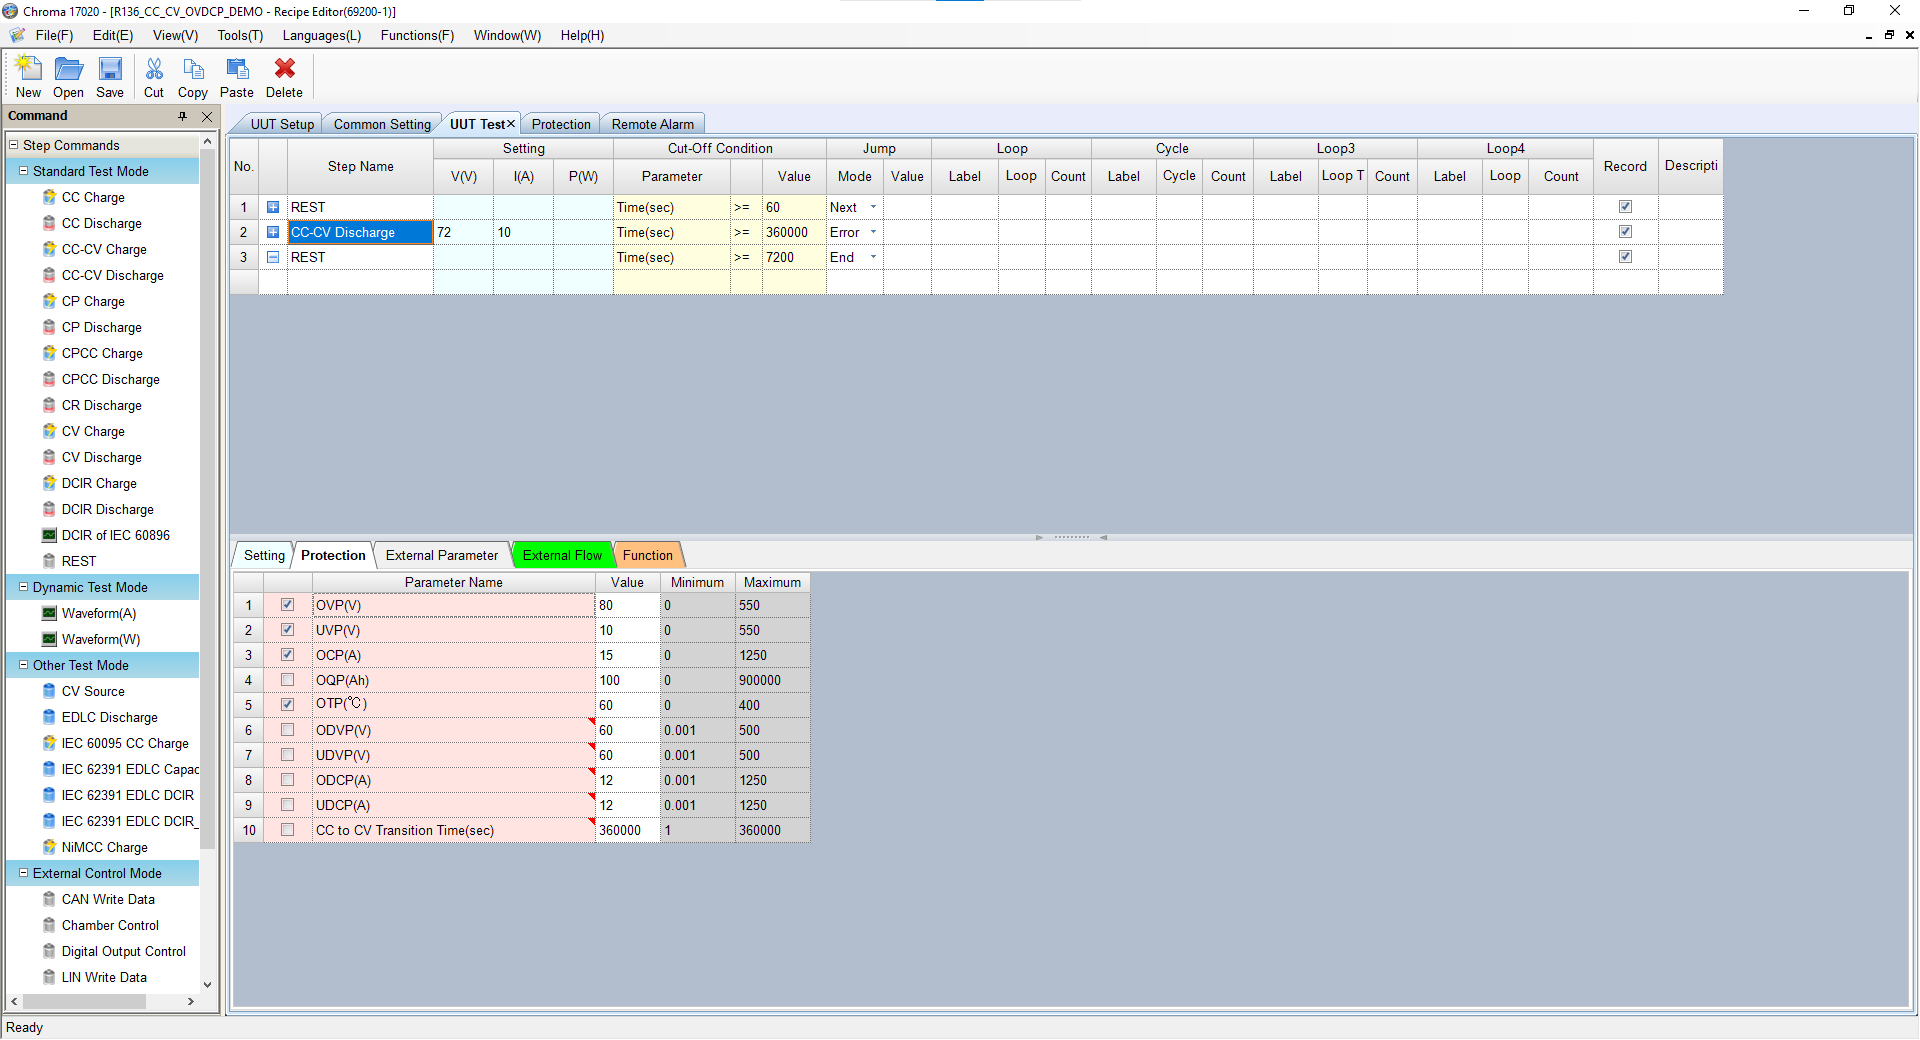
\includegraphics[width=1\linewidth]{Chapters/img/R136_DEMO/UUT_TEST_OVDCP.png}
		\centering
		\captionsetup{justification=centering,margin=2cm}
		\caption{การตั้งค่าสำหรับการทดสอบการป้องกันการดิสชาร์จเกินของแบตเตอรี่}
	\end{figure}
\end{center}
















